% template created by: Russell Haering. arr. Joseph Crop
\documentclass[12pt,letterpaper]{article}
\usepackage{anysize}
\usepackage{graphicx}
\usepackage{enumerate}
\marginsize{2cm}{2cm}{1cm}{1cm}

\begin{document}

\begin{titlepage}
    \vspace*{4cm}
    \begin{flushright}
    {\huge
        ECE 375 Homework 1\\[1cm]
    }
    {\large
       Computer Organization and Assembly Language Programming
    }
    \end{flushright}
    \begin{flushleft}
    Winter Term 2018
    \end{flushleft}
    \begin{flushright}
    Jeremy Fischer

    \end{flushright}

\end{titlepage}


\section{Homework Questions}
\begin{enumerate}
    %Question 1
    \item
    Consider a 1-address CPU that has a memory unit with 128K words of 32 bits each. 
    An instruction is stored in one memory word. 
    The instruction format is divided into four fields: an opcode field, a 2-bit addressing mode
    field that specify direct, indirect, indirect with pre-decrement, or indirect with post-increment addressing mode, a register field that specifies one of 32 registers, and an address field. 
    For your information, given an \textit{address}
    \begin{itemize}
        \item{Direct addressing is where the operand is located in M[\textit{address}].}
        \item{Indirect addressing is where the operand is located in M[M[\textit{address}]].}
        \item{Indirect addressing with pre-decrement is where the operand is located in M[-M[\textit{address}]].}
        \item{Indirect addressing with post-increment is where the operand is located in M[M[address]+].}
    \end{itemize}
	 \begin{enumerate}
        \item{What is the maximum number of opcodes that can be incorporated into the CPU? 
        	How many bits are in the opcode field, the register field, and the address field? 
        	Draw the instruction format and indicate the number of bits in each field.}
        
        \textbf{Answer:}
        
        The number of opcodes is 2\textsuperscript{K} where K is the number of bits occupied by a single opcode. Therefore, the number of opcodes is 2\textsuperscript{8} = 256 opcodes.
        
        \begin{figure}[h]
        	\centering
        	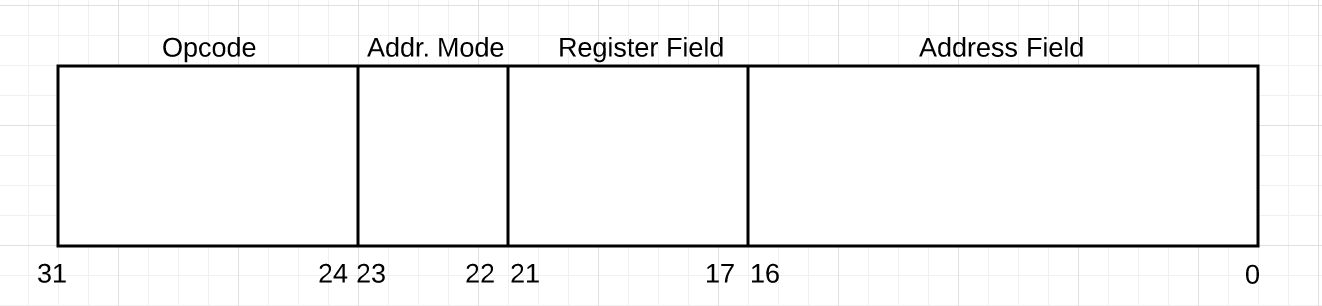
\includegraphics[width=0.65\textwidth]{Q1.png}
        \end{figure}
        
        
        \item{If this 1-address format is to be implemented on the pseudo-CPU discussed in class, how many bits are required for the registers PC, MAR, MDR, IR, and AC?}
        
        \textbf{Answer:}
        
        If we were using the CPU discussed in class then:
        
        PC: 13-bits because it holds an address, the address field of the CPU in class is 13-bits
        
        MAR: 13-bits because it holds an address, the address field of the CPU in class is 13-bits
        
        MDR: 16-bits because it holds words, a word in the CPU in class is 16-bits
        
        IR: 3-bits because it holds opcodes, an opcode in the CPU in class is 3-bits
        
        AC: 16-bits 
        
	\end{enumerate}

	
	






	\clearpage
	%Question 2
   \item
	Consider the following hypothetical 1-address assembly instruction called “Store Accumulator with Post-increment”
	of the form
	\begin{verbatim}
		STA (x)+  ; M(M(x)) <-- AC,    M(x) <-- M(x) + 1
	\end{verbatim}
	Suppose we want to implement this instruction on the pseudo-CPU discussed in class augmented with a
	temporary register TEMP. 
	An instruction consists of 16 bits: A 4-bit opcode and a 12-bit address. 
	All operands are 16 bits. 
	PC and MAR each contain 12 bits. 
	AC, MDR, and TEMP each contain 16 bits, and IR is 4 bits.
	Give the sequence of \textit{microoperations} required to implement the Execute cycle (Fetch cycle is given below) for
	the above STA (x)+ instruction. 
	Your solution should result in exactly 8 microoperations. 
	Assume PC is currently pointing to the STA (x)+ instruction and only PC and AC have the capability to increment/decrement
	itself. 
	\begin{figure}[h]
		\centering
		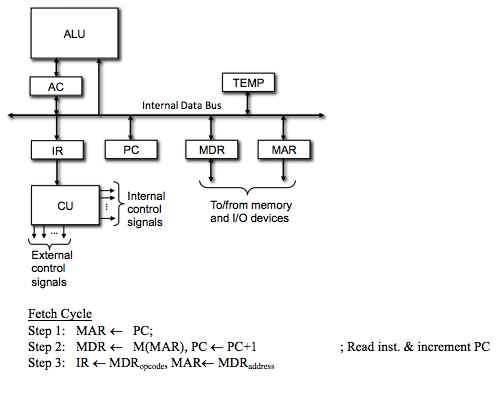
\includegraphics[width=0.6\textwidth]{Q2.png}
	\end{figure}

	\textbf{Answer:}
	
	Step 1: MDR $ \leftarrow$ AC 				\hfill ;move value to MDR	
	
	Step 2: TEMP $ \leftarrow$ MAR 	         \hfill ;store x so you can access later
	
	Step 3: M[M[MAR]] $ \leftarrow$ MDR  \hfill ;store value at M(M(x)) where x is held in MAR
	
	Step 4: AC $ \leftarrow$ M[MAR]		      \hfill  ;move M(x) to AC so M(x) can be incremented 
	
	Step 5: AC $ \leftarrow$ AC + 1 	       \hfill ;increment AC, M(x) + 1
	
	Step 6: MDR $ \leftarrow$ AC			   \hfill ;move M(x) + 1 to MDR
	
	Step 7: M[TEMP] $ \leftarrow$ MDR 	   \hfill ;store M(x) + 1  in M(x)
	
	Step 8: PC $ \leftarrow$ PC + 1				\hfill ;get the next instruction
	




	\clearpage
	%Question 3
	\item
	The PDP-8 was the first successful commercial minicomputer, produced by Digital Equipment Corporation
	(DEC) in the 1960s (see http://en.wikipedia.org/wiki/PDP-8). 
	One of the assembly instructions it supported was “Increment and Skip if Zero (ISZ)” of the form
	\begin{verbatim}
		ISZ Y ;		M(Y) <-- M(Y) + 1, 		If (M(Y) + 1 = 0) Then PC <-- PC + 1 
	\end{verbatim}
	Suppose the pseudo-CPU discussed in class with a temporary register (TEMP) shown below can be used to
	implement the ISZ instruction. 
	Give the sequence of \textit{microoperations} required to fetch and execute ISZ. 
	Your solution should result in minimum number of \textit{microoperations}. 
	You must not destroy the original content of the AC. 
	Assume PC is currently pointing to the instruction and only PC and AC have the capability to increment itself. 
	\begin{figure}[h]
		\centering
		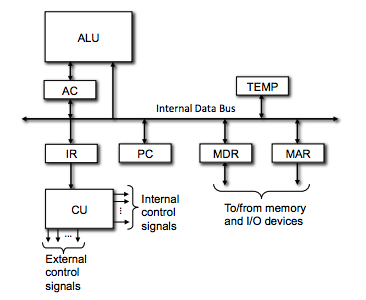
\includegraphics[width=0.6\textwidth]{Q3.png}
	\end{figure}
	
	\textbf{Answer:}
	
	Step 1: MAR $\leftarrow$ PC							\hfill ;move the instruction address to MAR
	
	Step 2: MDR $\leftarrow$ M[MAR]					\hfill ;move the opcode to MDR
	
	Step 3: IR $\leftarrow$ MDR\textsubscript{opcode}	\hfill ;load the instruction to IR to be decoded
	
	Step 4: MAR $\leftarrow$ MDR\textsubscript{address}  \hfill ;move Y to MAR
	
	Step 5: PC $\leftarrow$ PC + 1							\hfill ;increment PC to point to next instruction
	
	\centering \textit{Finished Fetching}
	
	Step 6: TEMP $\leftarrow$ AC 					\hfill ;store old value of AC
	
	Step 7: MDR $\leftarrow$ M[MAR]				\hfill ;MDR gets M(Y)
	
	Step 8: AC $\leftarrow$ MDR				  \hfill ;AC gets M(Y)
	
	Step 9: AC $\leftarrow$ AC + 1 					\hfill ;AC gets M(Y) + 1
	
	Step 10: MDR $\leftarrow$ AC 				\hfill ;MDR gets M(y) + 1
		
	Step 11: M[MAR] $\leftarrow$ MDR 				\hfill ;M(y) gets M(y) + 1
	
	\centering \textit{Finished Incrementing}
	
	Step 12: If (Z = 1) then PC $\leftarrow$ PC + 1 \hfill ;if Z = 1 last ALU operation was 0, skip
	
	Step 13: AC  $\leftarrow$ TEMP				\hfill ;move original AC value back to AC
	
	
	%Question 4
	\item
	Based on the initial register and data memory contents shown below (represented in hexadecimal), show how
	these contents are modified (in \textit{hexadecimal}) after executing each of the following AVR assembly instructions.
	Do not be concerned about what happens to the Status Register (SREG) \textit{after} the operation. 
	\textit{Instructions are unrelated}.

	\begin{figure}[h] %this figure will be at the right
		\flushright
		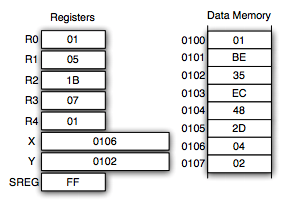
\includegraphics[width=0.4\textwidth]{Q4.png}
	\end{figure}
	
	\begin{enumerate}[i]
		\item{
			\begin{verbatim}
				CPI			R28, 2
			\end{verbatim}
			\textit{CPI compares the register and the immediate values}
			
			The operation (0x02 - 0x02) results in zero. Therefore, the Zero flag of SREG (bit 1) is set signifying that the two are equal.
		}
		\item{
			\begin{verbatim}
				STD			Y+0x05, R2
			\end{verbatim}
			\textit{STD stores contents of R\textsubscript{r} in indirect with displacement}
			
			After the operation data memory at 0x0107 has the value 0x1B
		}
		\item{
			\begin{verbatim}
				LD 			R3, -X
			\end{verbatim}
			\textit{LD loads indirect (\& with pre-decrement/post-increment)}
			
			After the operation R3 has the value 0x2D. X holds address 0106, but due to the pre-decrement, the real address we want is 0105, which holds 0x2D.
		}
		\item{
			\begin{verbatim}
				EOR 		R1, R3
			\end{verbatim}
			\textit{EOR is exclusive-OR}
			
			After the operation R1 has the value 0x02
		}
		\item{
			\begin{verbatim}
				SBIW 		R29:R28, 8
			\end{verbatim}
			\textit{SBIW subtracts an 8- bit value from a 16-bit register, such as X, Y or Z}
			
			After the operation R29:R28 is 0x00FA
		}
		\item{
			\begin{verbatim}
				SBR 		R26, 7
			\end{verbatim}
			\textit{SBR sets bits in a register}
			
			After the operation register R26 contains 0x07
		}
	\end{enumerate}
	
\end{enumerate}


       

\end{document}
